% DMA Session 6: Entity-Relationship-Modellierung
% 180-Minuten-Block (Vorlesung + Übung interwoven)

\documentclass[usenames,dvipsnames,10pt,aspectratio=169]{beamer}
\usepackage[T1]{fontenc}
\usepackage[utf8]{inputenc}
\usepackage{verbatim}

\usetheme{ims}

\usepackage{booktabs}
\usepackage{multicol}
\usepackage{listings}
\usepackage{xcolor}
\usepackage{graphicx}
\usepackage{tikz}
\usetikzlibrary{shapes.geometric, arrows.meta, positioning, calc, fit, backgrounds, er}
\usepackage{pifont}

% ER-Diagram TikZ styles
\tikzset{
    % Entity (rectangle)
    entity/.style={rectangle, draw=IMSBlue, fill=IMSBlue!10, thick,
        minimum width=2.5cm, minimum height=1cm, font=\bfseries},
    % Weak entity (double rectangle)
    weakentity/.style={rectangle, draw=IMSBlue, fill=IMSBlue!10, thick,
        minimum width=2.5cm, minimum height=1cm, font=\bfseries,
        double, double distance=2pt},
    % Relationship (diamond)
    relationship/.style={diamond, draw=IMSOrange, fill=IMSOrange!15, thick,
        minimum width=1.8cm, minimum height=1.2cm, aspect=2, font=\small},
    % Weak relationship
    weakrelationship/.style={diamond, draw=IMSOrange, fill=IMSOrange!15, thick,
        minimum width=1.8cm, minimum height=1.2cm, aspect=2, font=\small,
        double, double distance=2pt},
    % Attribute (ellipse)
    attribute/.style={ellipse, draw=gray!70, fill=gray!10,
        minimum width=1.5cm, minimum height=0.6cm, font=\small},
    % Key attribute (underlined)
    keyattribute/.style={ellipse, draw=gray!70, fill=gray!10,
        minimum width=1.5cm, minimum height=0.6cm, font=\small\underline},
    % Multivalued attribute (double ellipse)
    mvattribute/.style={ellipse, draw=gray!70, fill=gray!10,
        minimum width=1.5cm, minimum height=0.6cm, font=\small,
        double, double distance=1.5pt},
    % Derived attribute (dashed ellipse)
    derivedattribute/.style={ellipse, draw=gray!70, fill=gray!10, dashed,
        minimum width=1.5cm, minimum height=0.6cm, font=\small},
    % Cardinality label
    card/.style={font=\footnotesize, text=IMSBlue, align=center},
    % Connection line
    erline/.style={thick, gray!70},
    % Crow's foot styles
    crowone/.style={-{Tee[length=3mm, width=4mm]}, thick, gray!70},
    crowmany/.style={-{Straight Barb[left, length=2mm] Straight Barb[right, length=2mm]}, thick, gray!70},
    % Standard styles from previous sessions
    roadmapbox/.style={rectangle, rounded corners, minimum width=3cm, minimum height=1cm,
        text centered, draw=IMSBlue, fill=IMSBlue!10, font=\small\bfseries},
    roadmaparrow/.style={-{Stealth[length=3mm]}, thick, IMSBlue},
    % ISA triangle (apex points down toward subtypes)
    isatriangle/.style={isosceles triangle, draw=IMSBlue, fill=IMSBlue!10, thick,
        isosceles triangle apex angle=60, minimum width=1.2cm, shape border rotate=-90, font=\small},
}

% SQL Listing Style
\lstdefinestyle{sql}{
    language=SQL,
    basicstyle=\ttfamily\footnotesize,
    keywordstyle=\color{IMSBlue}\bfseries,
    stringstyle=\color{IMSOrange},
    commentstyle=\color{gray}\itshape,
    showstringspaces=false,
    breaklines=true,
    frame=single,
    backgroundcolor=\color{gray!10},
    morekeywords={SERIAL, BOOLEAN, TEXT, REFERENCES},
    literate={ü}{{\"u}}1 {ä}{{\"a}}1 {ö}{{\"o}}1 {Ü}{{\"U}}1 {Ä}{{\"A}}1 {Ö}{{\"O}}1 {ß}{{\ss}}1
}

\lstset{style=sql}

\newcommand{\cmark}{\textcolor{green!70!black}{\ding{51}}}
\newcommand{\xmark}{\textcolor{red}{\ding{55}}}

% ===== CLICKABLE AGENDA WITH PROGRESS INDICATOR =====
\usepackage{hyperref}
\hypersetup{colorlinks=false, pdfborder={0 0 0}}

% Phase counter for progress tracking
\newcounter{currentphase}
\setcounter{currentphase}{0}

% Clickable agenda item
\newcommand{\agendaitem}[3]{%
    \ifnum#1=#2
        \textcolor{IMSOrange}{$\blacktriangleright$ \textbf{\hyperlink{phase#2}{#3}}}%
    \else
        \textcolor{gray!70}{\phantom{$\blacktriangleright$} \hyperlink{phase#2}{#3}}%
    \fi\\[0.3em]%
}

% Progress dots for footline (clickable)
\newcommand{\progressdots}{%
    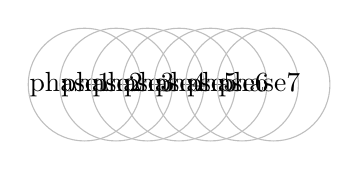
\begin{tikzpicture}[baseline=-0.5ex]
        \foreach \i in {1,...,7} {
            \ifnum\value{currentphase}=\i
                \node[circle, fill=IMSOrange, minimum size=0.24cm, inner sep=0pt] at (\i*0.4,0) {\hyperlink{phase\i}{\phantom{oo}}};
            \else
                \ifnum\value{currentphase}>\i
                    \node[circle, fill=IMSBlue!60, minimum size=0.2cm, inner sep=0pt] at (\i*0.4,0) {\hyperlink{phase\i}{\phantom{oo}}};
                \else
                    \node[circle, draw=gray!50, minimum size=0.2cm, inner sep=0pt] at (\i*0.4,0) {\hyperlink{phase\i}{\phantom{oo}}};
                \fi
            \fi
        }
    \end{tikzpicture}%
}

% Add progress indicator to footline
\setbeamertemplate{footline}{%
    \leavevmode%
    \hbox{%
        \begin{beamercolorbox}[wd=.33\paperwidth,ht=2.5ex,dp=1ex,left]{author in head/foot}%
            \usebeamerfont{author in head/foot}\hspace*{2ex}\insertshortauthor
        \end{beamercolorbox}%
        \begin{beamercolorbox}[wd=.34\paperwidth,ht=2.5ex,dp=1ex,center]{title in head/foot}%
            \progressdots
        \end{beamercolorbox}%
        \begin{beamercolorbox}[wd=.33\paperwidth,ht=2.5ex,dp=1ex,right]{date in head/foot}%
            \usebeamerfont{date in head/foot}\insertframenumber{} / \inserttotalframenumber\hspace*{2ex}
        \end{beamercolorbox}%
    }%
    \vskip0pt%
}

\newcommand{\showagenda}[1]{%
\setcounter{currentphase}{#1}%
\hypertarget{phase#1}{}%
\begin{frame}{Agenda}
\vfill
\begin{center}
\begin{minipage}{0.6\textwidth}
\large
\agendaitem{#1}{1}{1 ~ Rückblick \& Motivation}
\agendaitem{#1}{2}{2 ~ Entitäten \& Attribute}
\agendaitem{#1}{3}{3 ~ Beziehungen \& Kardinalitäten}
\agendaitem{#1}{4}{4 ~ Erweiterte Konzepte}
\agendaitem{#1}{5}{5 ~ Notationen im Vergleich}
\agendaitem{#1}{6}{6 ~ Modellierungspraxis}
\agendaitem{#1}{7}{7 ~ Zusammenfassung}
\end{minipage}
\end{center}
\vfill
\end{frame}
}

%%%%%%%%%%%%%%%%%%%%%%%%%%%%%%%%%%%%%%%%%%%%%%%%%%%%%%%%%%%%%%%%%%%%%%%%%%%%%%%%%%%%%
\title[DMA 06]{Datenmanagement \& -analyse}
\subtitle{Vorlesung 6: Entity-Relationship-Modellierung}
\author{Prof. Dr. Christoph M. Flath}
\institute{Lehrstuhl für Wirtschaftsinformatik und Business Analytics\\Julius-Maximilians-Universität Würzburg}
\date{Sommersemester 2026}
%%%%%%%%%%%%%%%%%%%%%%%%%%%%%%%%%%%%%%%%%%%%%%%%%%%%%%%%%%%%%%%%%%%%%%%%%%%%%%%%%%%%%

\begin{document}

% ===== TITLE =====
\begin{frame}[plain]
    \titlepage
\end{frame}

% ===== PHASE 1: Rückblick & Motivation =====
\showagenda{1}

\begin{frame}{Rückblick: Warum mehrere Tabellen?}
\begin{columns}[T]
\column{0.5\textwidth}
\textbf{Probleme der Mega-Tabelle:}
\begin{itemize}
    \item \textcolor{red}{Redundanz} -- gleiche Daten mehrfach
    \item \textcolor{red}{Änderungsanomalie} -- Inkonsistenzen
    \item \textcolor{red}{Einfügeanomalie} -- abhängige Daten
    \item \textcolor{red}{Löschanomalie} -- Datenverlust
\end{itemize}

\vspace{1em}
\textbf{Lösung:}\\
Daten auf mehrere Tabellen aufteilen!

\column{0.5\textwidth}
\begin{tikzpicture}[scale=0.8, transform shape]
    \node[roadmapbox] (prob) at (0,2) {Mega-Tabelle};
    \node[roadmapbox, fill=green!10, draw=green!50!black] (sol) at (0,0) {Mehrere Tabellen};
    \draw[roadmaparrow] (prob) -- (sol) node[midway, right, font=\small] {Aufteilen};
\end{tikzpicture}
\end{columns}
\end{frame}

\begin{frame}{Die zentrale Frage}
\begin{center}
\Huge\color{IMSBlue}
Wie wissen wir, welche Tabellen wir brauchen?
\end{center}

\vspace{2em}

\begin{center}
\Large
$\Rightarrow$ \textbf{Entity-Relationship-Modellierung}
\end{center}
\end{frame}

\begin{frame}{Was ist ein ER-Modell?}
\begin{columns}[T]
\column{0.55\textwidth}
\textbf{Entity-Relationship-Modell (ER-Modell):}
\begin{itemize}
    \item Grafische Notation für Datenstrukturen
    \item Entwickelt 1976 von Peter Chen
    \item Beschreibt die ``Welt'' in:
    \begin{itemize}
        \item \textbf{Entitäten} (Dinge)
        \item \textbf{Beziehungen} (Verbindungen)
        \item \textbf{Attributen} (Eigenschaften)
    \end{itemize}
    \item Unabhängig von der Datenbank
\end{itemize}

\column{0.45\textwidth}
\begin{tikzpicture}[scale=0.7, transform shape]
    \node[entity] (spieler) at (0,0) {Spieler};
    \node[entity] (verein) at (5,0) {Verein};
    \node[relationship] (spielt) at (2.5,0) {spielt für};
    \draw[erline] (spieler) -- (spielt);
    \draw[erline] (spielt) -- (verein);
\end{tikzpicture}

\vspace{1em}
\small\textit{Einfaches ER-Diagramm}
\end{columns}
\end{frame}

\begin{frame}{Warum ER-Modellierung?}
\begin{columns}[T]
\column{0.5\textwidth}
\textbf{Vorteile:}
\begin{itemize}
    \item \cmark{} Visuelle Kommunikation
    \item \cmark{} Gemeinsame Sprache mit Fachexperten
    \item \cmark{} Fehler früh erkennen
    \item \cmark{} Dokumentation der Datenstruktur
    \item \cmark{} Grundlage für SQL-Schema
\end{itemize}

\column{0.5\textwidth}
\textbf{Einsatzgebiete:}
\begin{itemize}
    \item Neue Datenbankprojekte
    \item Systemanalyse
    \item Requirements Engineering
    \item Reverse Engineering bestehender DBs
    \item Klausuren und Prüfungen
\end{itemize}
\end{columns}

\vspace{1em}
\begin{block}{Praxisrelevanz}
ER-Modelle sind Standard in der Softwareentwicklung -- jeder IT-Professional sollte sie lesen und erstellen können.
\end{block}
\end{frame}

\begin{frame}{Der Modellierungsprozess}
\begin{center}
\begin{tikzpicture}[node distance=1.5cm]
    \node[roadmapbox, minimum width=3.5cm] (real) {Reale Welt};
    \node[roadmapbox, minimum width=3.5cm, right=of real] (er) {ER-Modell};
    \node[roadmapbox, minimum width=3.5cm, right=of er] (rel) {Relationales Schema};
    \node[roadmapbox, minimum width=3.5cm, right=of rel] (sql) {SQL-Tabellen};

    \draw[roadmaparrow] (real) -- (er) node[midway, above, font=\footnotesize] {Analyse};
    \draw[roadmaparrow] (er) -- (rel) node[midway, above, font=\footnotesize] {Transformation};
    \draw[roadmaparrow] (rel) -- (sql) node[midway, above, font=\footnotesize] {CREATE TABLE};
\end{tikzpicture}
\end{center}

\vspace{1em}

\begin{itemize}
    \item \textbf{Heute:} Reale Welt $\rightarrow$ ER-Modell
    \item \textbf{Nächste Vorlesung:} ER-Modell $\rightarrow$ Relationales Schema
\end{itemize}
\end{frame}

% ===== PHASE 2: Entitäten & Attribute =====
\showagenda{2}

\begin{frame}{Entitäten (Entities)}
\begin{columns}[T]
\column{0.6\textwidth}
\textbf{Definition:}\\
Eine \textbf{Entität} ist ein unterscheidbares ``Ding'' der realen Welt.

\vspace{1em}
\textbf{Beispiele:}
\begin{itemize}
    \item Ein konkreter Spieler (Thomas Müller)
    \item Ein konkreter Verein (Bayern München)
    \item Eine konkrete Bestellung (\#12345)
\end{itemize}

\vspace{1em}
\textbf{Entitätstyp:}\\
Menge gleichartiger Entitäten\\
(z.B. ``alle Spieler'')

\column{0.4\textwidth}
\begin{tikzpicture}
    \node[entity] (spieler) {Spieler};
    \node[below=0.5cm of spieler, font=\small\itshape, text=gray] {Entitätstyp};

    \node[entity] (verein) at (0,-2.5) {Verein};
    \node[below=0.5cm of verein, font=\small\itshape, text=gray] {Entitätstyp};
\end{tikzpicture}
\end{columns}
\end{frame}

\begin{frame}{Entitäten identifizieren: Systematischer Ansatz}
\textbf{Schritt-für-Schritt:}

\vspace{0.5em}
\begin{enumerate}
    \item \textbf{Substantive markieren} in der Anforderungsbeschreibung
    \item \textbf{Filtern:} Welche sind eigenständige ``Dinge''?
    \item \textbf{Prüfen:} Haben sie eigene Eigenschaften?
    \item \textbf{Abgrenzen:} Sind sie von anderen unterscheidbar?
\end{enumerate}

\vspace{1em}
\textbf{Beispiel-Anforderung:}
\begin{quote}
``\underline{Kunden} bestellen \underline{Produkte}. Jeder \underline{Kunde} hat einen Namen und eine Adresse. \underline{Produkte} haben einen Preis und gehören zu einer \underline{Kategorie}.''
\end{quote}

\vspace{0.5em}
$\Rightarrow$ \textbf{Entitäten:} Kunde, Produkt, Kategorie

\vspace{0.5em}
$\Rightarrow$ \textbf{Keine Entitäten:} Name, Adresse, Preis (das sind Attribute!)
\end{frame}

\begin{frame}{Entität oder Attribut? -- Entscheidungshilfe}
\begin{columns}[T]
\column{0.5\textwidth}
\textbf{Eher Entität, wenn:}
\begin{itemize}
    \item Eigene Eigenschaften vorhanden
    \item Mehrere Beziehungen zu anderen
    \item Eigenständig speicherbar
    \item Mehrfach referenziert
\end{itemize}

\vspace{1em}
\textbf{Beispiel:}\\
``Adresse'' mit Straße, PLZ, Ort, Land\\
$\Rightarrow$ Entität (wenn wiederverwendet)

\column{0.5\textwidth}
\textbf{Eher Attribut, wenn:}
\begin{itemize}
    \item Nur ein Wert pro Entität
    \item Keine eigenen Beziehungen
    \item Einfacher Datentyp
    \item Gehört fest zur Entität
\end{itemize}

\vspace{1em}
\textbf{Beispiel:}\\
``Geburtsdatum'' eines Kunden\\
$\Rightarrow$ Attribut
\end{columns}

\vspace{1em}
\begin{alertblock}{Faustregel}
Im Zweifelsfall: Eher zu Entität tendieren. Refactoring zu Attribut ist einfacher als umgekehrt.
\end{alertblock}
\end{frame}

\begin{frame}{Attribute}
\textbf{Definition:}\\
\textbf{Attribute} beschreiben Eigenschaften von Entitäten oder Beziehungen.

\vspace{1em}
\begin{center}
\begin{tikzpicture}[scale=0.9, transform shape]
    \node[entity] (spieler) at (0,0) {Spieler};

    % Attributes
    \node[attribute] (name) at (-3,1.5) {Name};
    \node[attribute] (pos) at (0,2) {Position};
    \node[attribute] (alter) at (3,1.5) {Alter};
    \node[attribute] (id) at (-3,-1.5) {\underline{Spieler\_ID}};

    \draw[erline] (spieler) -- (name);
    \draw[erline] (spieler) -- (pos);
    \draw[erline] (spieler) -- (alter);
    \draw[erline] (spieler) -- (id);

    \node[below=0.3cm of id, font=\footnotesize, text=IMSBlue] {Schlüsselattribut};
\end{tikzpicture}
\end{center}
\end{frame}

\begin{frame}{Attributtypen}
\begin{columns}[T]
\column{0.5\textwidth}
\textbf{Einfache Attribute:}
\begin{itemize}
    \item Atomarer Wert (nicht teilbar)
    \item Beispiel: Alter, Punktzahl
\end{itemize}

\vspace{0.5em}
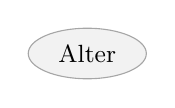
\begin{tikzpicture}
    \node[attribute] {Alter};
\end{tikzpicture}

\vspace{1em}
\textbf{Zusammengesetzte Attribute:}
\begin{itemize}
    \item Besteht aus Teilattributen
    \item Beispiel: Adresse (Straße, PLZ, Ort)
\end{itemize}

\vspace{0.5em}
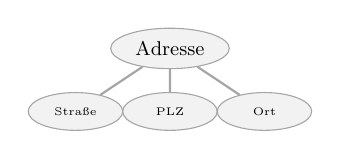
\begin{tikzpicture}[scale=0.8, transform shape]
    \node[attribute] (addr) at (0,0) {Adresse};
    \node[attribute, font=\tiny] (str) at (-1.5,-1) {Straße};
    \node[attribute, font=\tiny] (plz) at (0,-1) {PLZ};
    \node[attribute, font=\tiny] (ort) at (1.5,-1) {Ort};
    \draw[erline] (addr) -- (str);
    \draw[erline] (addr) -- (plz);
    \draw[erline] (addr) -- (ort);
\end{tikzpicture}

\column{0.5\textwidth}
\textbf{Mehrwertige Attribute:}
\begin{itemize}
    \item Mehrere Werte pro Entität
    \item Beispiel: Telefonnummern
\end{itemize}

\vspace{0.5em}
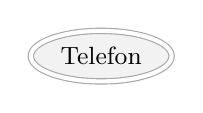
\begin{tikzpicture}
    \node[mvattribute] {Telefon};
\end{tikzpicture}

\vspace{1em}
\textbf{Abgeleitete Attribute:}
\begin{itemize}
    \item Berechenbar aus anderen
    \item Beispiel: Alter (aus Geburtsdatum)
\end{itemize}

\vspace{0.5em}
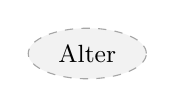
\begin{tikzpicture}
    \node[derivedattribute] {Alter};
\end{tikzpicture}
\end{columns}
\end{frame}

\begin{frame}{Schlüsselattribute}
\begin{columns}[T]
\column{0.6\textwidth}
\textbf{Schlüsselattribut:}
\begin{itemize}
    \item Identifiziert eine Entität eindeutig
    \item Wird \underline{unterstrichen} dargestellt
    \item Entspricht dem Primärschlüssel
\end{itemize}

\vspace{1em}
\textbf{Beispiele:}
\begin{itemize}
    \item \underline{Spieler\_ID}
    \item \underline{Verein\_ID}
    \item \underline{Matrikelnummer}
\end{itemize}

\vspace{1em}
\textbf{Zusammengesetzter Schlüssel:}\\
Mehrere Attribute zusammen bilden den Schlüssel

\column{0.4\textwidth}
\begin{tikzpicture}
    \node[entity] (spieler) at (0,0) {Spieler};
    \node[attribute] (id) at (0,1.8) {\underline{Spieler\_ID}};
    \node[attribute] (name) at (-2,0.8) {Name};
    \node[attribute] (pos) at (2,0.8) {Position};

    \draw[erline] (spieler) -- (id);
    \draw[erline] (spieler) -- (name);
    \draw[erline] (spieler) -- (pos);
\end{tikzpicture}
\end{columns}
\end{frame}

\begin{frame}{Starke vs. Schwache Entitäten}
\begin{columns}[T]
\column{0.5\textwidth}
\textbf{Starke Entität:}
\begin{itemize}
    \item Existiert unabhängig
    \item Hat eigenen Primärschlüssel
    \item Beispiel: Verein
\end{itemize}

\vspace{1em}
\begin{tikzpicture}
    \node[entity] (verein) {Verein};
\end{tikzpicture}

\column{0.5\textwidth}
\textbf{Schwache Entität:}
\begin{itemize}
    \item Existiert nur mit ``Owner''
    \item Braucht Fremdschlüssel zur Identifikation
    \item Beispiel: Raum (in einem Gebäude)
\end{itemize}

\vspace{1em}
\begin{tikzpicture}
    \node[weakentity] (raum) {Raum};
\end{tikzpicture}
\end{columns}

\vspace{1em}
\begin{alertblock}{Praxis}
Schwache Entitäten sind selten. Im Zweifelsfall: starke Entität mit eigenem Schlüssel.
\end{alertblock}
\end{frame}

\begin{frame}{Schwache Entitäten im Detail}
\begin{center}
\begin{tikzpicture}[scale=0.8, transform shape]
    \node[entity] (gebaeude) at (0,0) {Gebäude};
    \node[weakentity] (raum) at (6,0) {Raum};
    \node[weakrelationship] (liegt) at (3,0) {liegt in};

    % Attribute Gebäude
    \node[attribute, font=\tiny] at (-2,1.2) {\underline{Gebäude\_ID}};
    \node[attribute, font=\tiny] at (0,1.5) {Name};
    \node[attribute, font=\tiny] at (2,1.2) {Adresse};
    \draw[erline] (gebaeude) -- (-2,1.2);
    \draw[erline] (gebaeude) -- (0,1.5);
    \draw[erline] (gebaeude) -- (2,1.2);

    % Attribute Raum (partieller Schlüssel)
    \node[attribute, font=\tiny] at (6,1.5) {\underline{Raum\_Nr}};
    \node[attribute, font=\tiny] at (8,1) {Kapazität};
    \draw[erline] (raum) -- (6,1.5);
    \draw[erline] (raum) -- (8,1);

    \draw[erline, double] (gebaeude) -- (liegt) node[midway, above, card] {1};
    \draw[erline, double] (liegt) -- (raum) node[midway, above, card] {N};
\end{tikzpicture}
\end{center}

\vspace{1em}
\textbf{Eigenschaften schwacher Entitäten:}
\begin{itemize}
    \item \textbf{Partieller Schlüssel:} Raum\_Nr (nur innerhalb eines Gebäudes eindeutig)
    \item \textbf{Identifizierende Beziehung:} ``liegt in'' (doppelte Raute)
    \item \textbf{Vollständiger Schlüssel:} Gebäude\_ID + Raum\_Nr
\end{itemize}

\vspace{0.5em}
\textbf{Weitere Beispiele:} Kontozeile (in Konto), Bestellposition (in Bestellung), Stockwerk (in Gebäude)
\end{frame}

% ===== PHASE 3: Beziehungen & Kardinalitäten =====
\showagenda{3}

\begin{frame}{Beziehungen (Relationships)}
\begin{columns}[T]
\column{0.55\textwidth}
\textbf{Definition:}\\
Eine \textbf{Beziehung} (Relationship) beschreibt eine Verbindung zwischen Entitäten.

\vspace{1em}
\textbf{Beziehungstyp:}\\
Menge gleichartiger Beziehungen\\
(z.B. ``Spieler spielt für Verein'')

\vspace{1em}
\textbf{Darstellung:}\\
Raute (Diamond) zwischen Entitäten

\column{0.45\textwidth}
\begin{tikzpicture}[scale=0.8, transform shape]
    \node[entity] (spieler) at (0,0) {Spieler};
    \node[entity] (verein) at (5,0) {Verein};
    \node[relationship] (spielt) at (2.5,0) {spielt für};
    \draw[erline] (spieler) -- (spielt);
    \draw[erline] (spielt) -- (verein);
\end{tikzpicture}

\vspace{2em}
\small\textit{``Müller spielt für Bayern''}
\end{columns}
\end{frame}

\begin{frame}{Beziehungsgrade}
\begin{columns}[T]
\column{0.33\textwidth}
\textbf{Binär (Grad 2):}\\
Zwei Entitätstypen

\vspace{0.5em}
\begin{tikzpicture}[scale=0.6, transform shape]
    \node[entity] (a) at (0,0) {A};
    \node[entity] (b) at (4,0) {B};
    \node[relationship] (r) at (2,0) {R};
    \draw[erline] (a) -- (r);
    \draw[erline] (r) -- (b);
\end{tikzpicture}

\vspace{0.5em}
\small Spieler -- Verein

\column{0.33\textwidth}
\textbf{Unär (Grad 1):}\\
Ein Entitätstyp

\vspace{0.5em}
\begin{tikzpicture}[scale=0.6, transform shape]
    \node[entity] (a) at (0,0) {A};
    \node[relationship] (r) at (0,-2) {R};
    \draw[erline] (a.south west) -- (r.north west);
    \draw[erline] (a.south east) -- (r.north east);
\end{tikzpicture}

\vspace{0.5em}
\small Mitarbeiter -- Vorgesetzter

\column{0.33\textwidth}
\textbf{Ternär (Grad 3):}\\
Drei Entitätstypen

\vspace{0.5em}
\begin{tikzpicture}[scale=0.6, transform shape]
    \node[entity] (a) at (0,1) {A};
    \node[entity] (b) at (3,1) {B};
    \node[entity] (c) at (1.5,-1.5) {C};
    \node[relationship] (r) at (1.5,0) {R};
    \draw[erline] (a) -- (r);
    \draw[erline] (b) -- (r);
    \draw[erline] (c) -- (r);
\end{tikzpicture}

\vspace{0.5em}
\small Projekt -- Mitarbeiter -- Rolle
\end{columns}

\vspace{1em}
\begin{alertblock}{Praxis}
Binäre Beziehungen sind am häufigsten. Ternäre lassen sich oft in binäre zerlegen.
\end{alertblock}
\end{frame}

\begin{frame}{Beziehungsattribute}
Auch Beziehungen können Attribute haben:

\vspace{1em}
\begin{center}
\begin{tikzpicture}[scale=0.85, transform shape]
    \node[entity] (spieler) at (0,0) {Spieler};
    \node[entity] (verein) at (7,0) {Verein};
    \node[relationship] (spielt) at (3.5,0) {spielt für};

    \node[attribute] (von) at (3.5,1.8) {seit};
    \node[attribute] (bis) at (5.5,1.5) {Rückennr.};

    \draw[erline] (spieler) -- (spielt);
    \draw[erline] (spielt) -- (verein);
    \draw[erline] (spielt) -- (von);
    \draw[erline] (spielt) -- (bis);
\end{tikzpicture}
\end{center}

\vspace{1em}
\textbf{Typische Beziehungsattribute:}
\begin{itemize}
    \item Zeitangaben (seit, bis, Datum)
    \item Mengen (Anzahl, Stückzahl)
    \item Rollen (Position, Funktion)
\end{itemize}
\end{frame}

\begin{frame}{Kardinalitäten: Die Kernfrage}
\begin{center}
\Large
\textcolor{IMSBlue}{Wie viele} Entitäten auf der einen Seite\\
können mit \textcolor{IMSBlue}{wie vielen} auf der anderen verbunden sein?
\end{center}

\vspace{2em}

\begin{itemize}
    \item \textbf{1:1} -- Eins zu Eins
    \item \textbf{1:N} -- Eins zu Viele
    \item \textbf{M:N} -- Viele zu Viele
\end{itemize}
\end{frame}

\begin{frame}{Kardinalität 1:1 (Eins zu Eins)}
\textbf{Jede Entität auf einer Seite ist mit höchstens einer auf der anderen verbunden.}

\vspace{1em}
\begin{center}
\begin{tikzpicture}[scale=0.85, transform shape]
    \node[entity] (land) at (0,0) {Land};
    \node[entity] (hauptstadt) at (7,0) {Hauptstadt};
    \node[relationship] (hat) at (3.5,0) {hat};

    \draw[erline] (land) -- (hat) node[midway, above, card] {1};
    \draw[erline] (hat) -- (hauptstadt) node[midway, above, card] {1};
\end{tikzpicture}
\end{center}

\vspace{1em}
\textbf{Beispiele:}
\begin{itemize}
    \item Land -- Hauptstadt
    \item Person -- Personalausweis
    \item Mitarbeiter -- Parkplatz (falls jeder max. einen hat)
\end{itemize}

\begin{alertblock}{Hinweis}
1:1-Beziehungen sind selten. Oft könnte man die Entitäten zusammenlegen.
\end{alertblock}
\end{frame}

\begin{frame}{Kardinalität 1:1 -- Wann sinnvoll?}
\textbf{Gründe für separate Entitäten trotz 1:1:}

\vspace{1em}
\begin{columns}[T]
\column{0.5\textwidth}
\begin{enumerate}
    \item \textbf{Optionalität:}\\
    Nicht jeder Mitarbeiter hat Firmenwagen

    \vspace{0.5em}
    \item \textbf{Unterschiedliche Lebenszyklen:}\\
    Personalausweis wird erneuert

    \vspace{0.5em}
    \item \textbf{Viele Attribute:}\\
    Trennung für Übersichtlichkeit
\end{enumerate}

\column{0.5\textwidth}
\begin{tikzpicture}[scale=0.7, transform shape]
    \node[entity] (ma) at (0,0) {Mitarbeiter};
    \node[entity] (fw) at (0,-3) {Firmenwagen};
    \node[relationship] (hat) at (0,-1.5) {fährt};

    \draw[erline] (ma) -- (hat) node[midway, right, card] {(0,1)};
    \draw[erline] (hat) -- (fw) node[midway, right, card] {(0,1)};
\end{tikzpicture}

\small\textit{Nicht jeder hat einen,\\nicht jeder Wagen ist zugeteilt}
\end{columns}
\end{frame}

\begin{frame}{Kardinalität 1:N (Eins zu Viele)}
\textbf{Eine Entität auf einer Seite kann mit vielen auf der anderen verbunden sein.}

\vspace{1em}
\begin{center}
\begin{tikzpicture}[scale=0.85, transform shape]
    \node[entity] (verein) at (0,0) {Verein};
    \node[entity] (spieler) at (7,0) {Spieler};
    \node[relationship] (hat) at (3.5,0) {hat};

    \draw[erline] (verein) -- (hat) node[midway, above, card] {1};
    \draw[erline] (hat) -- (spieler) node[midway, above, card] {N};
\end{tikzpicture}
\end{center}

\vspace{1em}
\textbf{Beispiele:}
\begin{itemize}
    \item Verein -- Spieler (ein Spieler, ein Verein)
    \item Abteilung -- Mitarbeiter
    \item Kunde -- Bestellungen
    \item Mutter -- Kinder
\end{itemize}

\begin{block}{Häufigste Kardinalität!}
Die meisten Beziehungen in der Praxis sind 1:N.
\end{block}
\end{frame}

\begin{frame}{1:N Beispiele aus der Praxis}
\begin{columns}[T]
\column{0.5\textwidth}
\textbf{E-Commerce:}
\begin{tikzpicture}[scale=0.6, transform shape]
    \node[entity] (kunde) at (0,0) {Kunde};
    \node[entity] (bestellung) at (0,-2.5) {Bestellung};
    \node[relationship] (r) at (0,-1.25) {gibt auf};
    \draw[erline] (kunde) -- (r) node[midway, right, card] {1};
    \draw[erline] (r) -- (bestellung) node[midway, right, card] {N};
\end{tikzpicture}

\vspace{1em}
\textbf{Universität:}
\begin{tikzpicture}[scale=0.6, transform shape]
    \node[entity] (prof) at (0,0) {Professor};
    \node[entity] (vorl) at (0,-2.5) {Vorlesung};
    \node[relationship] (r) at (0,-1.25) {hält};
    \draw[erline] (prof) -- (r) node[midway, right, card] {1};
    \draw[erline] (r) -- (vorl) node[midway, right, card] {N};
\end{tikzpicture}

\column{0.5\textwidth}
\textbf{Unternehmen:}
\begin{tikzpicture}[scale=0.6, transform shape]
    \node[entity] (abt) at (0,0) {Abteilung};
    \node[entity] (ma) at (0,-2.5) {Mitarbeiter};
    \node[relationship] (r) at (0,-1.25) {beschäftigt};
    \draw[erline] (abt) -- (r) node[midway, right, card] {1};
    \draw[erline] (r) -- (ma) node[midway, right, card] {N};
\end{tikzpicture}

\vspace{1em}
\textbf{Bibliothek:}
\begin{tikzpicture}[scale=0.6, transform shape]
    \node[entity] (autor) at (0,0) {Verlag};
    \node[entity] (buch) at (0,-2.5) {Buch};
    \node[relationship] (r) at (0,-1.25) {veröffentlicht};
    \draw[erline] (autor) -- (r) node[midway, right, card] {1};
    \draw[erline] (r) -- (buch) node[midway, right, card] {N};
\end{tikzpicture}
\end{columns}
\end{frame}

\begin{frame}{Kardinalität M:N (Viele zu Viele)}
\textbf{Entitäten auf beiden Seiten können mit vielen auf der anderen verbunden sein.}

\vspace{1em}
\begin{center}
\begin{tikzpicture}[scale=0.85, transform shape]
    \node[entity] (student) at (0,0) {Student};
    \node[entity] (kurs) at (7,0) {Kurs};
    \node[relationship] (besucht) at (3.5,0) {besucht};

    \draw[erline] (student) -- (besucht) node[midway, above, card] {M};
    \draw[erline] (besucht) -- (kurs) node[midway, above, card] {N};
\end{tikzpicture}
\end{center}

\vspace{1em}
\textbf{Beispiele:}
\begin{itemize}
    \item Student -- Kurs (viele Studenten, viele Kurse)
    \item Autor -- Buch (Co-Autoren)
    \item Schauspieler -- Film
    \item Produkt -- Zutat (Rezepte)
\end{itemize}
\end{frame}

\begin{frame}{M:N mit Beziehungsattributen}
\textbf{M:N-Beziehungen haben oft eigene Attribute:}

\vspace{1em}
\begin{center}
\begin{tikzpicture}[scale=0.8, transform shape]
    \node[entity] (student) at (0,0) {Student};
    \node[entity] (kurs) at (7,0) {Kurs};
    \node[relationship] (nimmt) at (3.5,0) {nimmt teil};

    \node[attribute, font=\tiny] at (3.5,1.8) {Note};
    \node[attribute, font=\tiny] at (5.2,1.5) {Semester};

    \draw[erline] (student) -- (nimmt) node[midway, above, card] {M};
    \draw[erline] (nimmt) -- (kurs) node[midway, above, card] {N};
    \draw[erline] (nimmt) -- (3.5,1.8);
    \draw[erline] (nimmt) -- (5.2,1.5);
\end{tikzpicture}
\end{center}

\vspace{1em}
\textbf{Weitere Beispiele mit Attributen:}
\begin{itemize}
    \item Mitarbeiter -- Projekt: \textit{Rolle, Stunden, Zeitraum}
    \item Schauspieler -- Film: \textit{Rolle, Gage}
    \item Lieferant -- Produkt: \textit{Preis, Lieferzeit}
\end{itemize}

\begin{block}{Wichtig}
M:N-Beziehungen werden bei der Transformation zu eigenen Tabellen!
\end{block}
\end{frame}

\begin{frame}{(Min,Max)-Notation}
\textbf{Genauere Angabe der Kardinalitäten:}

\vspace{1em}
\begin{center}
\begin{tikzpicture}[scale=0.85, transform shape]
    \node[entity] (verein) at (0,0) {Verein};
    \node[entity] (spieler) at (7,0) {Spieler};
    \node[relationship] (hat) at (3.5,0) {hat};

    \draw[erline] (verein) -- (hat) node[midway, above, card] {(11,30)};
    \draw[erline] (hat) -- (spieler) node[midway, above, card] {(1,1)};
\end{tikzpicture}
\end{center}

\vspace{1em}
\textbf{Bedeutung:}
\begin{itemize}
    \item (11,30) bei Verein: Ein Verein hat 11 bis 30 Spieler
    \item (1,1) bei Spieler: Ein Spieler gehört zu genau 1 Verein
\end{itemize}

\vspace{1em}
\textbf{Spezialfälle:}
\begin{itemize}
    \item (0,1) -- optional, höchstens einer
    \item (1,1) -- genau einer (Pflicht)
    \item (0,N) oder (0,*) -- optional, beliebig viele
    \item (1,N) oder (1,*) -- mindestens einer, beliebig viele
\end{itemize}
\end{frame}

\begin{frame}{Quiz: Welche Kardinalität? (1/2)}
\textbf{Bestimmen Sie die Kardinalität:}

\vspace{1em}
\begin{enumerate}
    \item \textbf{Buch -- Verlag}
    \begin{itemize}
        \item Ein Buch erscheint bei einem Verlag
        \item Ein Verlag veröffentlicht viele Bücher
        \item $\Rightarrow$ \pause \textcolor{IMSBlue}{\textbf{1:N}} (Verlag:Buch)
    \end{itemize}

    \pause
    \vspace{0.5em}
    \item \textbf{Patient -- Arzt}
    \begin{itemize}
        \item Ein Patient kann mehrere Ärzte haben
        \item Ein Arzt behandelt mehrere Patienten
        \item $\Rightarrow$ \pause \textcolor{IMSBlue}{\textbf{M:N}}
    \end{itemize}

    \pause
    \vspace{0.5em}
    \item \textbf{Auto -- Kennzeichen} (in Deutschland)
    \begin{itemize}
        \item Ein Auto hat genau ein Kennzeichen
        \item Ein Kennzeichen gehört zu genau einem Auto
        \item $\Rightarrow$ \pause \textcolor{IMSBlue}{\textbf{1:1}}
    \end{itemize}
\end{enumerate}
\end{frame}

\begin{frame}{Quiz: Welche Kardinalität? (2/2)}
\textbf{Bestimmen Sie die Kardinalität:}

\vspace{1em}
\begin{enumerate}
    \setcounter{enumi}{3}
    \item \textbf{Ehepartner -- Ehepartner} (aktuell, monogam)
    \begin{itemize}
        \item Eine Person hat höchstens einen Ehepartner
        \item $\Rightarrow$ \pause \textcolor{IMSBlue}{\textbf{1:1 unär (rekursiv)}}
    \end{itemize}

    \pause
    \vspace{0.5em}
    \item \textbf{Rezept -- Zutat}
    \begin{itemize}
        \item Ein Rezept enthält mehrere Zutaten
        \item Eine Zutat kommt in mehreren Rezepten vor
        \item $\Rightarrow$ \pause \textcolor{IMSBlue}{\textbf{M:N}} (mit Attribut ``Menge''!)
    \end{itemize}

    \pause
    \vspace{0.5em}
    \item \textbf{Mitarbeiter -- Vorgesetzter}
    \begin{itemize}
        \item Ein Mitarbeiter hat einen Vorgesetzten
        \item Ein Vorgesetzter hat mehrere Mitarbeiter
        \item $\Rightarrow$ \pause \textcolor{IMSBlue}{\textbf{1:N unär (rekursiv)}}
    \end{itemize}
\end{enumerate}
\end{frame}

% ===== PAUSE =====
\begin{frame}[plain]
\vfill
\begin{center}
{\Huge Pause}\\[0.5em]
{\large 15 Minuten}
\end{center}
\vfill
\end{frame}

% ===== PHASE 4: Erweiterte Konzepte =====
\showagenda{4}

\begin{frame}{Rekursive Beziehungen (Unär)}
\textbf{Eine Entität steht in Beziehung zu sich selbst:}

\vspace{1em}
\begin{center}
\begin{tikzpicture}[scale=0.8, transform shape]
    \node[entity] (ma) at (0,0) {Mitarbeiter};
    \node[relationship] (r) at (0,-2.5) {ist Vorgesetzter};

    \draw[erline] (ma.south west) to[out=-120, in=150] node[midway, left, card] {0..1\\Vorgesetzter} (r.north west);
    \draw[erline] (ma.south east) to[out=-60, in=30] node[midway, right, card] {0..N\\Mitarbeiter} (r.north east);
\end{tikzpicture}
\end{center}

\vspace{1em}
\textbf{Weitere Beispiele rekursiver Beziehungen:}
\begin{itemize}
    \item Person -- ``ist verheiratet mit'' -- Person (1:1)
    \item Produkt -- ``ist Ersatzteil für'' -- Produkt (M:N)
    \item Kategorie -- ``ist Unterkategorie von'' -- Kategorie (1:N)
\end{itemize}
\end{frame}

\begin{frame}{ISA-Hierarchie (Generalisierung/Spezialisierung)}
\textbf{Vererbungsbeziehung zwischen Entitätstypen:}

\vspace{1em}
\begin{center}
\begin{tikzpicture}[scale=0.75, transform shape]
    % Supertype
    \node[entity] (person) at (0,2) {Person};
    \node[attribute, font=\tiny] at (-2.5,3) {\underline{Person\_ID}};
    \node[attribute, font=\tiny] at (0,3.3) {Name};
    \node[attribute, font=\tiny] at (2.5,3) {Geburtsdatum};
    \draw[erline] (person) -- (-2.5,3);
    \draw[erline] (person) -- (0,3.3);
    \draw[erline] (person) -- (2.5,3);

    % ISA
    \node[isatriangle] (isa) at (0,0.5) {ISA};

    % Subtypes
    \node[entity] (student) at (-3,-1.5) {Student};
    \node[entity] (dozent) at (3,-1.5) {Dozent};

    \node[attribute, font=\tiny] at (-5,-1.5) {Matrikel\_Nr};
    \node[attribute, font=\tiny] at (-3,-3) {Semester};
    \draw[erline] (student) -- (-5,-1.5);
    \draw[erline] (student) -- (-3,-3);

    \node[attribute, font=\tiny] at (5,-1.5) {Personal\_Nr};
    \node[attribute, font=\tiny] at (3,-3) {Fachgebiet};
    \draw[erline] (dozent) -- (5,-1.5);
    \draw[erline] (dozent) -- (3,-3);

    \draw[erline] (person) -- (isa);
    \draw[erline] (isa) -- (student);
    \draw[erline] (isa) -- (dozent);
\end{tikzpicture}
\end{center}

\vspace{0.5em}
\textbf{Bedeutung:} Student \textit{ist eine} Person, Dozent \textit{ist eine} Person
\end{frame}

\begin{frame}{ISA: Overlapping vs. Disjoint}
\begin{columns}[T]
\column{0.5\textwidth}
\textbf{Disjoint (disjunkt):}
\begin{itemize}
    \item Entität gehört zu \textbf{höchstens einem} Subtyp
    \item Markierung: ``d'' im Dreieck
\end{itemize}

\vspace{0.5em}
\begin{tikzpicture}[scale=0.6, transform shape]
    \node[entity] (fahrzeug) at (0,2) {Fahrzeug};
    \node[isatriangle, minimum width=1cm, font=\footnotesize] (isa) at (0,0.5) {d};
    \node[entity, minimum width=1.8cm] (pkw) at (-2,-1) {PKW};
    \node[entity, minimum width=1.8cm] (lkw) at (2,-1) {LKW};
    \draw[erline] (fahrzeug) -- (isa);
    \draw[erline] (isa) -- (pkw);
    \draw[erline] (isa) -- (lkw);
\end{tikzpicture}

\small Ein Fahrzeug ist PKW \textbf{oder} LKW

\column{0.5\textwidth}
\textbf{Overlapping (überlappend):}
\begin{itemize}
    \item Entität kann zu \textbf{mehreren} Subtypen gehören
    \item Markierung: ``o'' im Dreieck
\end{itemize}

\vspace{0.5em}
\begin{tikzpicture}[scale=0.6, transform shape]
    \node[entity] (person) at (0,2) {Person};
    \node[isatriangle, minimum width=1cm, font=\footnotesize] (isa) at (0,0.5) {o};
    \node[entity, minimum width=1.8cm] (stud) at (-2,-1) {Student};
    \node[entity, minimum width=1.8cm] (ma) at (2,-1) {Mitarbeiter};
    \draw[erline] (person) -- (isa);
    \draw[erline] (isa) -- (stud);
    \draw[erline] (isa) -- (ma);
\end{tikzpicture}

\small HiWi ist Student \textbf{und} Mitarbeiter
\end{columns}
\end{frame}

\begin{frame}{ISA: Total vs. Partial}
\begin{columns}[T]
\column{0.5\textwidth}
\textbf{Total (vollständig):}
\begin{itemize}
    \item Jede Entität gehört zu \textbf{mindestens einem} Subtyp
    \item Doppelte Linie zum ISA
\end{itemize}

\vspace{0.5em}
\begin{tikzpicture}[scale=0.6, transform shape]
    \node[entity] (konto) at (0,2) {Konto};
    \node[isatriangle, minimum width=1cm, font=\footnotesize] (isa) at (0,0.5) {d};
    \node[entity, minimum width=1.5cm, font=\small\bfseries] (giro) at (-2,-1) {Giro};
    \node[entity, minimum width=1.5cm, font=\small\bfseries] (spar) at (2,-1) {Spar};
    \draw[erline, double] (konto) -- (isa);
    \draw[erline] (isa) -- (giro);
    \draw[erline] (isa) -- (spar);
\end{tikzpicture}

\small Jedes Konto \textbf{muss} Giro oder Spar sein

\column{0.5\textwidth}
\textbf{Partial (partiell):}
\begin{itemize}
    \item Entität muss \textbf{nicht} zu einem Subtyp gehören
    \item Einfache Linie zum ISA
\end{itemize}

\vspace{0.5em}
\begin{tikzpicture}[scale=0.6, transform shape]
    \node[entity] (person) at (0,2) {Person};
    \node[isatriangle, minimum width=1cm, font=\footnotesize] (isa) at (0,0.5) {d};
    \node[entity, minimum width=1.5cm, font=\small\bfseries] (stud) at (-2,-1) {Student};
    \node[entity, minimum width=1.5cm, font=\small\bfseries] (prof) at (2,-1) {Professor};
    \draw[erline] (person) -- (isa);
    \draw[erline] (isa) -- (stud);
    \draw[erline] (isa) -- (prof);
\end{tikzpicture}

\small Person kann auch ``nur Person'' sein
\end{columns}

\vspace{1em}
\begin{block}{Kombination}
Die vier Varianten kombinieren: \textbf{disjoint/total}, \textbf{disjoint/partial}, \textbf{overlapping/total}, \textbf{overlapping/partial}
\end{block}
\end{frame}

% ===== PHASE 5: Notationen =====
\showagenda{5}

\begin{frame}{Notationen im Überblick}
\textbf{Es gibt verschiedene ER-Notationen:}

\vspace{1em}
\begin{tabular}{lll}
\toprule
\textbf{Notation} & \textbf{Erfinder/Quelle} & \textbf{Einsatz} \\
\midrule
Chen-Notation & Peter Chen (1976) & Lehre, Theorie \\
Crow's Foot & verschiedene & UML, Praxis-Tools \\
(Min,Max) & verschiedene & Präzise Constraints \\
UML-Klassendiagramm & OMG & Software Engineering \\
\bottomrule
\end{tabular}

\vspace{1em}
\begin{alertblock}{Wichtig}
Alle Notationen drücken dasselbe aus -- nur die Symbole unterscheiden sich!
\end{alertblock}
\end{frame}

\begin{frame}{Chen-Notation (Klassisch)}
\begin{center}
\begin{tikzpicture}[scale=0.7, transform shape]
    % Legende
    \node[entity] at (0,3) {Entität};
    \node[right, font=\small] at (1.8,3) {Starke Entität (Rechteck)};

    \node[weakentity] at (0,1.5) {Schwach};
    \node[right, font=\small] at (1.8,1.5) {Schwache Entität (Doppelrechteck)};

    \node[relationship] at (0,0) {Bez.};
    \node[right, font=\small] at (1.8,0) {Beziehung (Raute)};

    \node[attribute] at (0,-1.5) {Attr};
    \node[right, font=\small] at (1.8,-1.5) {Attribut (Ellipse)};

    \node[attribute] at (0,-3) {\underline{Key}};
    \node[right, font=\small] at (1.8,-3) {Schlüsselattribut (unterstrichen)};

    \node[mvattribute] at (7,3) {Multi};
    \node[right, font=\small] at (8.8,3) {Mehrwertig (Doppelellipse)};

    \node[derivedattribute] at (7,1.5) {Abgel.};
    \node[right, font=\small] at (8.8,1.5) {Abgeleitet (gestrichelt)};

    % Kardinalitäten
    \node[font=\small\bfseries] at (7,-0.5) {Kardinalitäten:};
    \node[font=\small] at (7,-1.5) {1:1, 1:N, M:N};
    \node[font=\small] at (7,-2.5) {oder (min,max)};
\end{tikzpicture}
\end{center}
\end{frame}

\begin{frame}{Crow's Foot Notation}
\textbf{In Praxis-Tools (ERwin, Visio, MySQL Workbench) weit verbreitet:}

\vspace{1em}
\begin{center}
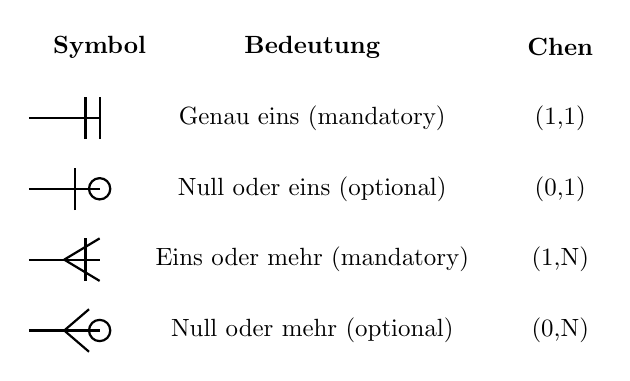
\begin{tikzpicture}[scale=0.9, transform shape]
    % Symbole erklären
    \node[font=\bfseries] at (-3, 2) {Symbol};
    \node[font=\bfseries] at (0, 2) {Bedeutung};
    \node[font=\bfseries] at (3.5, 2) {Chen};

    % One mandatory
    \draw[thick] (-4,1) -- (-3,1);
    \draw[thick] (-3.2,0.7) -- (-3.2,1.3);
    \draw[thick] (-3,0.7) -- (-3,1.3);
    \node at (0,1) {Genau eins (mandatory)};
    \node at (3.5,1) {(1,1)};

    % One optional
    \draw[thick] (-4,0) -- (-3,0);
    \draw[thick] (-3,0) circle (0.15);
    \draw[thick] (-3.35,-0.3) -- (-3.35,0.3);
    \node at (0,0) {Null oder eins (optional)};
    \node at (3.5,0) {(0,1)};

    % Many mandatory
    \draw[thick] (-4,-1) -- (-3,-1);
    \draw[thick] (-3.2,-1.3) -- (-3.2,-0.7);
    \draw[thick] (-3.5,-1) -- (-3,-0.7);
    \draw[thick] (-3.5,-1) -- (-3,-1.3);
    \node at (0,-1) {Eins oder mehr (mandatory)};
    \node at (3.5,-1) {(1,N)};

    % Many optional
    \draw[thick] (-4,-2) -- (-3,-2);
    \draw[thick] (-3,-2) circle (0.15);
    \draw[thick] (-3.5,-2) -- (-3.15,-1.7);
    \draw[thick] (-3.5,-2) -- (-3.15,-2.3);
    \node at (0,-2) {Null oder mehr (optional)};
    \node at (3.5,-2) {(0,N)};
\end{tikzpicture}
\end{center}
\end{frame}

\begin{frame}{Chen vs. Crow's Foot -- Beispiel}
\textbf{Dieselbe Beziehung in beiden Notationen:}

\vspace{1em}
\begin{columns}[T]
\column{0.5\textwidth}
\textbf{Chen-Notation:}
\begin{center}
\begin{tikzpicture}[scale=0.65, transform shape]
    \node[entity] (verein) at (0,0) {Verein};
    \node[entity] (spieler) at (5,0) {Spieler};
    \node[relationship] (hat) at (2.5,0) {hat};
    \draw[erline] (verein) -- (hat) node[midway, above, card] {1};
    \draw[erline] (hat) -- (spieler) node[midway, above, card] {N};
\end{tikzpicture}
\end{center}

\vspace{0.5em}
\small Ein Verein hat viele Spieler,\\ein Spieler gehört zu einem Verein.

\column{0.5\textwidth}
\textbf{Crow's Foot Notation:}
\begin{center}
\begin{tikzpicture}[scale=0.65, transform shape]
    \node[entity] (verein) at (0,0) {Verein};
    \node[entity] (spieler) at (5,0) {Spieler};

    % Connection with crow's foot
    \draw[thick, gray!70] (verein) -- (spieler);
    % One side (Verein)
    \draw[thick, gray!70] (1.1,-0.3) -- (1.1,0.3);
    \draw[thick, gray!70] (1.3,-0.3) -- (1.3,0.3);
    % Many side (Spieler) - crow's foot
    \draw[thick, gray!70] (3.9,-0.3) -- (3.9,0.3);
    \draw[thick, gray!70] (3.5,0) -- (3.9,-0.3);
    \draw[thick, gray!70] (3.5,0) -- (3.9,0.3);
\end{tikzpicture}
\end{center}

\vspace{0.5em}
\small Dieselbe Semantik,\\kompaktere Darstellung.
\end{columns}

\vspace{1em}
\begin{block}{Empfehlung}
In der Klausur: Chen-Notation verwenden (expliziter, weniger fehleranfällig).\\
In der Praxis: Notation des verwendeten Tools nutzen.
\end{block}
\end{frame}

\begin{frame}{Vergleich: M:N in beiden Notationen}
\begin{columns}[T]
\column{0.5\textwidth}
\textbf{Chen-Notation:}
\begin{center}
\begin{tikzpicture}[scale=0.6, transform shape]
    \node[entity] (student) at (0,0) {Student};
    \node[entity] (kurs) at (5,0) {Kurs};
    \node[relationship] (besucht) at (2.5,0) {besucht};
    \node[attribute, font=\tiny] at (2.5,1.5) {Note};

    \draw[erline] (student) -- (besucht) node[midway, above, card] {M};
    \draw[erline] (besucht) -- (kurs) node[midway, above, card] {N};
    \draw[erline] (besucht) -- (2.5,1.5);
\end{tikzpicture}
\end{center}

\column{0.5\textwidth}
\textbf{Crow's Foot (mit Assoziationstabelle):}
\begin{center}
\begin{tikzpicture}[scale=0.6, transform shape]
    \node[entity] (student) at (0,0) {Student};
    \node[entity, minimum width=2cm] (teilnahme) at (3,0) {Teilnahme};
    \node[entity] (kurs) at (6,0) {Kurs};

    % Student - Teilnahme
    \draw[thick, gray!70] (student) -- (teilnahme);
    \draw[thick, gray!70] (1.1,-0.2) -- (1.1,0.2);
    \draw[thick, gray!70] (1.8,0) -- (2.1,-0.2);
    \draw[thick, gray!70] (1.8,0) -- (2.1,0.2);

    % Teilnahme - Kurs (many at Teilnahme, one at Kurs)
    \draw[thick, gray!70] (teilnahme) -- (kurs);
    \draw[thick, gray!70] (4.2,0) -- (3.9,-0.2);
    \draw[thick, gray!70] (4.2,0) -- (3.9,0.2);
    \draw[thick, gray!70] (4.9,-0.2) -- (4.9,0.2);

    \node[font=\tiny] at (3,-0.8) {Note};
\end{tikzpicture}
\end{center}
\end{columns}

\vspace{1em}
\textbf{Wichtiger Unterschied:}
\begin{itemize}
    \item Chen: M:N als Beziehung mit Attributen
    \item Crow's Foot: M:N wird zu Assoziations-Entität aufgelöst
\end{itemize}
\end{frame}

% ===== PHASE 6: Modellierungspraxis =====
\showagenda{6}

\begin{frame}{Modellierungsbeispiel: Online-Shop}
\textbf{Anforderungsbeschreibung:}

\vspace{0.5em}
\begin{quote}
``Ein Online-Shop verkauft Produkte an Kunden. Jeder Kunde hat einen Namen und eine E-Mail-Adresse. Produkte haben einen Namen, einen Preis und gehören zu einer Kategorie. Kunden können Bestellungen aufgeben, die mehrere Produkte enthalten können.''
\end{quote}

\vspace{1em}
\textbf{Schritt 1: Entitäten identifizieren}
\begin{itemize}
    \item Kunde
    \item Produkt
    \item Kategorie
    \item Bestellung
\end{itemize}
\end{frame}

\begin{frame}{Modellierungsbeispiel: Schritt 2 -- Attribute}
\begin{center}
\begin{tikzpicture}[scale=0.7, transform shape]
    % Kunde
    \node[entity] (kunde) at (0,3) {Kunde};
    \node[attribute, font=\tiny] at (-2,4.5) {\underline{Kunden\_ID}};
    \node[attribute, font=\tiny] at (0,4.8) {Name};
    \node[attribute, font=\tiny] at (2,4.5) {E-Mail};
    \draw[erline] (kunde) -- (-2,4.5);
    \draw[erline] (kunde) -- (0,4.8);
    \draw[erline] (kunde) -- (2,4.5);

    % Produkt
    \node[entity] (produkt) at (8,3) {Produkt};
    \node[attribute, font=\tiny] at (6,4.5) {\underline{Produkt\_ID}};
    \node[attribute, font=\tiny] at (8,4.8) {Name};
    \node[attribute, font=\tiny] at (10,4.5) {Preis};
    \draw[erline] (produkt) -- (6,4.5);
    \draw[erline] (produkt) -- (8,4.8);
    \draw[erline] (produkt) -- (10,4.5);

    % Kategorie
    \node[entity] (kat) at (8,-1) {Kategorie};
    \node[attribute, font=\tiny] at (10.5,-1) {\underline{Kat\_ID}};
    \node[attribute, font=\tiny] at (8,-2.5) {Name};
    \draw[erline] (kat) -- (10.5,-1);
    \draw[erline] (kat) -- (8,-2.5);

    % Bestellung
    \node[entity] (best) at (0,-1) {Bestellung};
    \node[attribute, font=\tiny] at (-2.5,-1) {\underline{Best\_ID}};
    \node[attribute, font=\tiny] at (0,-2.5) {Datum};
    \draw[erline] (best) -- (-2.5,-1);
    \draw[erline] (best) -- (0,-2.5);
\end{tikzpicture}
\end{center}
\end{frame}

\begin{frame}{Modellierungsbeispiel: Schritt 3 -- Beziehungen}
\begin{center}
\begin{tikzpicture}[scale=0.65, transform shape]
    % Entitäten
    \node[entity] (kunde) at (0,3) {Kunde};
    \node[entity] (best) at (0,0) {Bestellung};
    \node[entity] (produkt) at (6,0) {Produkt};
    \node[entity] (kat) at (6,-3) {Kategorie};

    % Beziehungen
    \node[relationship] (gibt) at (0,1.5) {gibt auf};
    \node[relationship] (enthaelt) at (3,0) {enthält};
    \node[relationship] (gehoert) at (6,-1.5) {gehört zu};

    % Verbindungen mit Kardinalitäten
    \draw[erline] (kunde) -- (gibt) node[midway, left, card] {1};
    \draw[erline] (gibt) -- (best) node[midway, left, card] {N};

    \draw[erline] (best) -- (enthaelt) node[midway, above, card] {M};
    \draw[erline] (enthaelt) -- (produkt) node[midway, above, card] {N};

    \draw[erline] (produkt) -- (gehoert) node[midway, left, card] {N};
    \draw[erline] (gehoert) -- (kat) node[midway, left, card] {1};

    % Beziehungsattribut
    \node[attribute, font=\tiny] at (3,1.3) {Menge};
    \draw[erline] (enthaelt) -- (3,1.3);
\end{tikzpicture}
\end{center}

\vspace{0.5em}
\textbf{Kardinalitäten:}
\begin{itemize}
    \item Kunde -- Bestellung: 1:N (ein Kunde, viele Bestellungen)
    \item Bestellung -- Produkt: M:N (mit Attribut ``Menge'')
    \item Produkt -- Kategorie: N:1 (viele Produkte, eine Kategorie)
\end{itemize}
\end{frame}

\begin{frame}{Vollständiges ER-Diagramm}
\begin{center}
\begin{tikzpicture}[scale=0.55, transform shape]
    % Kunde
    \node[entity] (kunde) at (0,4) {Kunde};
    \node[attribute, font=\tiny] at (-2,5.5) {\underline{ID}};
    \node[attribute, font=\tiny] at (0,5.8) {Name};
    \node[attribute, font=\tiny] at (2,5.5) {E-Mail};
    \draw[erline] (kunde) -- (-2,5.5);
    \draw[erline] (kunde) -- (0,5.8);
    \draw[erline] (kunde) -- (2,5.5);

    % Bestellung
    \node[entity] (best) at (0,0) {Bestellung};
    \node[attribute, font=\tiny] at (-2.5,0) {\underline{ID}};
    \node[attribute, font=\tiny] at (0,-1.5) {Datum};
    \draw[erline] (best) -- (-2.5,0);
    \draw[erline] (best) -- (0,-1.5);

    % Produkt
    \node[entity] (produkt) at (7,0) {Produkt};
    \node[attribute, font=\tiny] at (5,1.5) {\underline{ID}};
    \node[attribute, font=\tiny] at (7,1.8) {Name};
    \node[attribute, font=\tiny] at (9,1.5) {Preis};
    \draw[erline] (produkt) -- (5,1.5);
    \draw[erline] (produkt) -- (7,1.8);
    \draw[erline] (produkt) -- (9,1.5);

    % Kategorie
    \node[entity] (kat) at (7,-4) {Kategorie};
    \node[attribute, font=\tiny] at (9,-4) {\underline{ID}};
    \node[attribute, font=\tiny] at (7,-5.5) {Name};
    \draw[erline] (kat) -- (9,-4);
    \draw[erline] (kat) -- (7,-5.5);

    % Beziehungen
    \node[relationship] (gibt) at (0,2) {gibt auf};
    \node[relationship] (enthaelt) at (3.5,0) {enthält};
    \node[relationship] (gehoert) at (7,-2) {gehört zu};

    % Verbindungen
    \draw[erline] (kunde) -- (gibt) node[midway, left, card] {1};
    \draw[erline] (gibt) -- (best) node[midway, left, card] {N};

    \draw[erline] (best) -- (enthaelt) node[midway, above, card] {M};
    \draw[erline] (enthaelt) -- (produkt) node[midway, above, card] {N};
    \node[attribute, font=\tiny] at (3.5,1.3) {Menge};
    \draw[erline] (enthaelt) -- (3.5,1.3);

    \draw[erline] (produkt) -- (gehoert) node[midway, left, card] {N};
    \draw[erline] (gehoert) -- (kat) node[midway, left, card] {1};
\end{tikzpicture}
\end{center}
\end{frame}

\begin{frame}{Komplexes Beispiel: Universitätsverwaltung}
\begin{center}
\begin{tikzpicture}[scale=0.5, transform shape]
    % Entitäten
    \node[entity] (prof) at (0,4) {Professor};
    \node[entity] (vorl) at (5,4) {Vorlesung};
    \node[entity] (stud) at (10,4) {Student};
    \node[entity] (fak) at (0,0) {Fakultät};
    \node[entity] (pruef) at (5,0) {Prüfung};

    % ISA für Person (vereinfacht)

    % Beziehungen
    \node[relationship, font=\tiny] (haelt) at (2.5,4) {hält};
    \node[relationship, font=\tiny] (besucht) at (7.5,4) {besucht};
    \node[relationship, font=\tiny] (gehoert) at (0,2) {gehört zu};
    \node[relationship, font=\tiny] (schreibt) at (7.5,0) {schreibt};
    \node[relationship, font=\tiny] (zuvorl) at (5,2) {für};

    % Verbindungen
    \draw[erline] (prof) -- (haelt) node[midway, above, card] {1};
    \draw[erline] (haelt) -- (vorl) node[midway, above, card] {N};

    \draw[erline] (vorl) -- (besucht) node[midway, above, card] {M};
    \draw[erline] (besucht) -- (stud) node[midway, above, card] {N};

    \draw[erline] (prof) -- (gehoert) node[midway, left, card] {N};
    \draw[erline] (gehoert) -- (fak) node[midway, left, card] {1};

    \draw[erline] (stud) -- (schreibt) node[midway, right, card] {M};
    \draw[erline] (schreibt) -- (pruef) node[midway, above, card] {N};

    \draw[erline] (vorl) -- (zuvorl) node[midway, left, card] {1};
    \draw[erline] (zuvorl) -- (pruef) node[midway, left, card] {N};

    % Beziehungsattribute
    \node[attribute, font=\tiny] at (7.5,5.2) {Semester};
    \draw[erline] (besucht) -- (7.5,5.2);

    \node[attribute, font=\tiny] at (9,0) {Note};
    \draw[erline] (schreibt) -- (9,0);
\end{tikzpicture}
\end{center}

\vspace{0.5em}
\small\textbf{Beziehungen:} Professor hält Vorlesungen (1:N), Studenten besuchen Vorlesungen (M:N), Studenten schreiben Prüfungen zu Vorlesungen (M:N mit Attribut Note)
\end{frame}

\begin{frame}{Häufige Modellierungsfehler}
\begin{columns}[T]
\column{0.5\textwidth}
\textbf{Fehler vermeiden:}

\vspace{0.5em}
\xmark{} \textbf{Kardinalität verwechselt}
\begin{itemize}
    \item ``N bei Kunde'' statt ``N bei Bestellung''
    \item Tipp: Immer prüfen -- ``Ein X hat wie viele Y?''
\end{itemize}

\vspace{0.5em}
\xmark{} \textbf{Attribut statt Entität}
\begin{itemize}
    \item ``Kategoriename'' als Attribut von Produkt
    \item Tipp: Hat es eigene Attribute/Beziehungen?
\end{itemize}

\vspace{0.5em}
\xmark{} \textbf{M:N nicht erkannt}
\begin{itemize}
    \item ``Student hat einen Kurs'' (falsch!)
    \item Tipp: Beide Richtungen prüfen
\end{itemize}

\column{0.5\textwidth}
\textbf{Noch mehr Fehler:}

\vspace{0.5em}
\xmark{} \textbf{Schlüssel vergessen}
\begin{itemize}
    \item Jede Entität braucht Schlüsselattribut
\end{itemize}

\vspace{0.5em}
\xmark{} \textbf{Beziehungsattribute vergessen}
\begin{itemize}
    \item ``Menge'' bei Bestellung-Produkt
    \item ``Note'' bei Student-Prüfung
\end{itemize}

\vspace{0.5em}
\xmark{} \textbf{Redundante Beziehungen}
\begin{itemize}
    \item Direkter Pfad reicht meist
    \item Keine ``Abkürzungen'' einbauen
\end{itemize}
\end{columns}
\end{frame}

\begin{frame}{Best Practices für ER-Modellierung}
\begin{columns}[T]
\column{0.5\textwidth}
\textbf{Prozess:}
\begin{enumerate}
    \item Substantive $\rightarrow$ Entitäten
    \item Verben $\rightarrow$ Beziehungen
    \item Adjektive $\rightarrow$ Attribute
    \item Kardinalitäten bestimmen
    \item Schlüssel festlegen
    \item Review mit Stakeholdern
\end{enumerate}

\column{0.5\textwidth}
\textbf{Qualitätskriterien:}
\begin{itemize}
    \item \cmark{} Vollständig (alle Anforderungen)
    \item \cmark{} Redundanzfrei
    \item \cmark{} Konsistent (Namenskonventionen)
    \item \cmark{} Lesbar (gutes Layout)
    \item \cmark{} Dokumentiert (Glossar)
\end{itemize}
\end{columns}

\vspace{1em}
\begin{block}{Goldene Regel}
\textbf{Ein gutes ER-Modell ist für Fachexperten verständlich!}\\
Wenn der Kunde es nicht versteht, ist es zu kompliziert.
\end{block}
\end{frame}

% ===== Hands-on =====
{
\setbeamercolor{background canvas}{bg=IMSOrange!15}
\begin{frame}[plain]
\vfill
\begin{center}
{\Huge\color{IMSOrange} Hands-on}\\[1em]
{\Large Eigenes ER-Diagramm erstellen}\\[2em]
{\large Papier oder draw.io}\\[1em]
{\normalsize Aufgaben 6.1 -- 6.4}
\end{center}
\vfill
\end{frame}
}

\begin{frame}{Übungsaufgabe 6.1: Bibliothek}
\textbf{Erstellen Sie ein ER-Diagramm für eine Bibliothek:}

\vspace{0.5em}
\begin{quote}
``Eine Bibliothek verleiht Bücher an Mitglieder. Jedes Buch hat einen Titel, ISBN und einen oder mehrere Autoren. Mitglieder haben einen Namen und eine Mitgliedsnummer. Ein Buch kann mehrfach vorhanden sein (Exemplare). Mitglieder können Bücher ausleihen.''
\end{quote}

\vspace{1em}
\textbf{Hinweise:}
\begin{itemize}
    \item Identifizieren Sie die Entitäten
    \item Bestimmen Sie die Attribute (inkl. Schlüssel)
    \item Zeichnen Sie die Beziehungen mit Kardinalitäten
    \item Achtung: Buch vs. Exemplar!
\end{itemize}
\end{frame}

\begin{frame}{Übungsaufgabe 6.2: Universität}
\textbf{Erstellen Sie ein ER-Diagramm für eine Universität:}

\vspace{0.5em}
\begin{quote}
``Professoren halten Vorlesungen. Studierende besuchen Vorlesungen und schreiben Prüfungen. Jede Prüfung gehört zu einer Vorlesung. Studierende können mehrere Prüfungen ablegen.''
\end{quote}

\vspace{1em}
\textbf{Entitäten:}
\begin{itemize}
    \item Professor
    \item Vorlesung
    \item Student
    \item Prüfung (?)
\end{itemize}

\vspace{0.5em}
\textbf{Diskussion:} Ist ``Prüfung'' eine Entität oder eine Beziehung?
\end{frame}

\begin{frame}{Übungsaufgabe 6.3: Fitness-Studio}
\textbf{Erstellen Sie ein ER-Diagramm für ein Fitness-Studio:}

\vspace{0.5em}
\begin{quote}
``Ein Fitness-Studio bietet Kurse an, die von Trainern geleitet werden. Mitglieder können sich für Kurse anmelden. Kurse finden in bestimmten Räumen statt. Trainer können mehrere Kurse leiten. Mitglieder haben verschiedene Mitgliedschaftstypen (Basic, Premium, VIP).''
\end{quote}

\vspace{1em}
\textbf{Besondere Herausforderungen:}
\begin{itemize}
    \item Ist ``Mitgliedschaftstyp'' eine Entität oder Attribut?
    \item Welche Beziehungsattribute gibt es?
    \item Verwenden Sie (min,max)-Notation für Präzision
\end{itemize}
\end{frame}

\begin{frame}{Übungsaufgabe 6.4: Klausuraufgabe}
\textbf{Lieferplattform (aus Klausur SS2025):}

\vspace{0.5em}
\begin{quote}
``Ein Unternehmen betreibt eine Plattform, über die Restaurants Mahlzeiten liefern. Restaurants haben Kennung, Name und Adresse. Gerichte gehören zu Restaurants und haben Preis, Kalorien und Allergene. Kunden haben Kennung, Kontaktdaten und Unverträglichkeiten. Bestellungen enthalten mehrere Positionen (Gericht + Menge).''
\end{quote}

\vspace{1em}
\textbf{Aufgabe:}
\begin{itemize}
    \item Vollständiges ER-Diagramm
    \item (Min,Max)-Kardinalitäten
    \item Alle Attribute mit Schlüsseln
\end{itemize}
\end{frame}

% ===== PHASE 7: Zusammenfassung =====
\showagenda{7}

\begin{frame}{Zusammenfassung}
\begin{columns}[T]
\column{0.5\textwidth}
\textbf{ER-Modellierung:}
\begin{itemize}
    \item Grafische Darstellung von Datenstrukturen
    \item Unabhängig von der Implementierung
    \item Kommunikationsmittel mit Fachexperten
\end{itemize}

\vspace{1em}
\textbf{Kernelemente:}
\begin{itemize}
    \item \textbf{Entitäten} -- ``Dinge''
    \item \textbf{Attribute} -- Eigenschaften
    \item \textbf{Beziehungen} -- Verbindungen
    \item \textbf{Kardinalitäten} -- Anzahl
\end{itemize}

\column{0.5\textwidth}
\textbf{Modellierungsschritte:}
\begin{enumerate}
    \item Entitäten identifizieren
    \item Attribute zuordnen
    \item Schlüssel festlegen
    \item Beziehungen definieren
    \item Kardinalitäten bestimmen
\end{enumerate}

\vspace{1em}
\textbf{Erweiterte Konzepte:}
\begin{itemize}
    \item Schwache Entitäten
    \item ISA-Hierarchien
    \item Rekursive Beziehungen
\end{itemize}
\end{columns}
\end{frame}

\begin{frame}{Checkliste: ER-Diagramm prüfen}
\begin{columns}[T]
\column{0.5\textwidth}
\textbf{Vollständigkeit:}
\begin{itemize}
    \item[$\square$] Alle Entitäten aus Anforderung?
    \item[$\square$] Alle Attribute zugeordnet?
    \item[$\square$] Alle Beziehungen modelliert?
    \item[$\square$] Schlüsselattribute markiert?
\end{itemize}

\vspace{1em}
\textbf{Korrektheit:}
\begin{itemize}
    \item[$\square$] Kardinalitäten korrekt?
    \item[$\square$] Keine redundanten Beziehungen?
    \item[$\square$] Attribute am richtigen Ort?
\end{itemize}

\column{0.5\textwidth}
\textbf{Qualität:}
\begin{itemize}
    \item[$\square$] Einheitliche Namensgebung?
    \item[$\square$] Übersichtliches Layout?
    \item[$\square$] Keine kreuzenden Linien?
\end{itemize}

\vspace{1em}
\textbf{Validierung:}
\begin{itemize}
    \item[$\square$] Beispieldaten durchspielen
    \item[$\square$] Fachexperten befragen
    \item[$\square$] Grenzfälle prüfen
\end{itemize}
\end{columns}
\end{frame}

\begin{frame}{Ausblick: Nächste Vorlesung}
\textbf{Vorlesung 7: Relationales Modell \& Transformation}

\vspace{1em}
\begin{itemize}
    \item ER-Modell $\rightarrow$ Relationales Schema
    \item Transformationsregeln
    \item CREATE TABLE mit Schlüsseln
    \item Fremdschlüssel-Constraints
\end{itemize}

\vspace{2em}
\begin{center}
\begin{tikzpicture}[scale=0.7, transform shape]
    \node[entity] (e) at (0,0) {Entität};
    \node[roadmapbox, minimum width=3cm] (t) at (5,0) {CREATE TABLE};
    \draw[roadmaparrow] (e) -- (t) node[midway, above, font=\small] {Transformation};
\end{tikzpicture}
\end{center}
\end{frame}

\begin{frame}[plain]
\vfill
\begin{center}
{\Huge Fragen?}\\[2em]
{\large christoph.flath@uni-wuerzburg.de}
\end{center}
\vfill
\end{frame}

\end{document}
